\documentclass[a4paper]{article}

\usepackage[margin = 3cm]{geometry}
\usepackage{amsmath, amssymb}
\usepackage{float}
\usepackage[T1]{fontenc}
\usepackage{graphicx}
\usepackage{listings}
\usepackage{xcolor}
\usepackage{hyperref}

\lstset{%
    %backgroundcolor=\color{yellow!20},%
    basicstyle=\ttfamily%
    }%
    
\newcommand{\boldn}{\boldsymbol{n}}

\newcommand{\red}[1]{\textcolor{red}{#1}}

\begin{document}
 
\title{\red{VEMcomp: A MATLAB tool for semilinear parabolic PDEs in 2D and 3D}}
\author{Massimo Frittelli, Anotida Madzvamuse, Ivonne Sgura}

\maketitle

\begin{abstract}
\red{We present a Virtual Element MATLAB solver for elliptic or parabolic, linear or semilinear PDEs in two or three space dimensions., which we call VEMcomp. The library covers PDEs posed on different geometries, such as bulk, surface, or bulk-surface PDE probems. The solver employs the Virtual Element Method of lowest polynomial order $k=1$ on general polygonal or polyhedral meshes.  VEMcomp has three purposes.
First,  for special geometries,  VEMcomp generates polygonal and polyhedral meshes optimized for fast matrix assembly. Second, given a mesh for the considered geometry, possibly generated with an external program, VEMcomp computes all the matrices of the method.
Third, for multiple classes of PDEs, surface and bulk-surface PDEs,  VEMcomp solves the considered PDE problem with the Virtual Element method with a user-friendly interface.  An extensive set of examples illustrates the usage of the library and the optimal convergence rate of the method.}
\end{abstract}

\section{\red{Introduction}}


\red{The Virtual Element Method (VEM) was first proposed in \cite{beirao2013basic} for elliptic problems in two space dimensions as a generalization of the Finite Element Method, where the mesh elements can be general polygons instead of triangles.  The usage of polygons with arbitrarily many edges is made possible by enriching the local space of polynomials with suitable non-polynomial functions defined as solutions of an element-wise problem.  This elegant idea ensures the optimal polynomial accuracy of the method.\\
The immediate success of VEM is due to the multiple benefits of its geometric flexibility. Among such benefits, we mention: (i) efficient mesh refinement techniques \cite{cangiani2017posteriori, van2022mesh}, (ii) numerical solutions with high global regularity \cite{da2020c1,da2014virtual}, (iii) accurate approximation of boundaries 
\cite{da2019virtual, bertoluzza2019high, dassi2022bend},  (iv) easy mesh pasting \cite{da2018virtual, frittelli2018virtual}, and (v) easy handling of complex domain shapes and cuts \cite{benedetto2014virtual, dassi2022virtual}.\\
Motivated by its multiple benefits, the VEM was quickly extended to numerous PDE problems and applications. A non-exhaustive list of models for which VEMs are now available comprises (i) linear elliptic problems in two \cite{beirao2013basic, da2019virtual} and three \cite{da2017high} space dimensions,  (ii) semilinear elliptic problems in two or three space dimensions \cite{xiao2022nonconforming}, (iii) linear heat equation in two \cite{vacca2015virtual} and three \cite{zhao2019nonconforming} space dimensions, (iv) semilinear parabolic equations \cite{adak2019convergence} and reaction-diffusion systems \cite{huang2021posteriori}, (v) elasticity \cite{da2013virtual, gain2014virtual} and plasticity \cite{aldakheel2019virtual} problems,  (vi) phase-field models \cite{aldakheel2018phase, antonietti2016c}, (vii) fluid dynamics \cite{adak2021virtual, beirao2019stokes},
(viii) fracture models \cite{benedetto2014virtual},  and recently
(ix) surface \cite{bachini2021arbitrary, frittelli2018virtual} and bulk-surface \cite{frittelli2021bulk,  frittelli2023bsrds} PDEs.\\
%
Over ten years of its existence, the VEM has established itself as a reliable technology with desirable properties. This has stimulated the development of the first open-source VEM libraries and codes.  Here will will recall some of these libraries.  The  work in \cite{Sutton_2016} presents a MATLAB implementation of the baseline VEM application: the lowest order VEM for the Poisson problem in 2D. For the same problem, a high order VEM code in MATLAB is then provided in \cite{Herrera_2022}. An Abaqus-MATLAB VEM code for coupled thermo-elasticity problems in 2D is presented in \cite{Dhanush_2018}.  VEM libraries for elasticity problems in 2D are available in MATLAB/Octave \cite{VEMLAB} and C++ \cite{Ortiz_Bernardin_2019}. All the mentioned libraries are dedicated to specific use cases or applications and are confined to the two space dimensional setting. \\
To the best of the authors' knowledge, there is no open-source VEM library so far for PDE problems in three space dimensions and/or of surface or bulk-surface type. In this work,  we contribute to the field of VEM open-source libraries. We propose a MATLAB library,  which we call VEMcomp, for elliptic and parabolic PDE problems in 2D and 3D, including bulk, surface and bulk-surface PDE problems.  VEMcomp has three purposes:
\begin{enumerate}
\item For special geometries, both in 2D and 3D, such as rectangles, ellipses, parallelepipeds and ellipsoids, the library generates polygonal and polyhedral meshes specifically optimized for fast matrix assembly, following \cite{frittelli2021bulk, frittelli2023bsrds};
\item Given any polygonal or polyhedral mesh -not necessarily generated with VEMcomp itself-, the library generates all the matrices involved in the method (e.g. mass, stiffness).  For polygonal mesh generation, it is worth recalling the MATLAB library \texttt{PolyMesher} \cite{Talischi_2012};
\item For multiple classes of PDE problems,  the library performs matrix assembly and provides a black-box interface that allows the user to set the problem parameters, and returns the VEM numerical solution. For time-dependent problems, the time discretization is carried out with the Implicit-Explicit (IMEX) Euler method,  which is proven to be simple and effective in combination with FEMs and VEMs for surface \cite{Frittelli2017preserving, Frittelli2017cross} and bulk-surface PDEs \cite{frittelli2021bulk, frittelli2023bsrds}.
\end{enumerate}
%
The structure of the paper is as follows. In Section \ref{sec:overview} we state the multiple model problems to be addressed in this work, thereby motivating the functionalities of VEMcomp.  In Section \ref{sec:mesh_generation} we illustrate the VEMcomp facility for polygonal and polyhedral mesh generation. Section \ref{sec:computation_local_matrices} presents two classes of VEMcomp dedicated to the computation of local VEM matrices. In Section \ref{sec:user_friendly_solver} we showcase VEMcomp's user-friendly solver for the model problems outlined in Section \ref{sec:overview}. Section \ref{sec:numerical_examples} showcases several numerical examples that illustrate at once the usage of VEMcomp and the optimal convergence of the Virtual Element Method.}



\section{\red{Overview}}
\label{sec:overview}
\red{VEMcomp is an object-oriented VEM library written in MATLAB.  Compared to other existing VEM libraries, VEMcomp aims to fill the gap for (i) PDE problems in three space dimensions and (ii) PDE problems on complex geometries, such as surface or bulk-surface PDEs. In the remainder of this section, let $\Omega \subset \mathbb{R}^d$, $d=2,3$, be a compact domain in the $d$-dimensional Euclidean space.  The first class of PDE problems covered by VEMcomp comprises elliptic and parabolic, linear and semilinear, bulk-only PDE systems of $n\in\mathbb{N}$ equations, and is given by
\begin{equation}
\label{bulk_only_problem}
\begin{cases}
\left[\dfrac{\partial u_i}{\partial t}\right] - d_i^\Omega\Delta u_i = f_i(u_1,\dots, u_n, \bold x, [t]), \qquad \bold x \in \Omega \qquad  i=1,\dots,n;\\
u_{i} = 0 \quad \text{or} \quad \dfrac{\partial u_i}{\partial \bold n} = 0,  \qquad \bold x \in \partial \Omega\qquad  i=1,\dots,n,
\end{cases}
\end{equation}
where $\Delta$ denotes the Laplace operator in $\Omega$, $d_1^\Omega,\dots, d_n^\Omega > 0$ are diffusion coefficients $T>0$ is the final time, $f_1, \dots, f_n$ are smooth enough linear or nonlinear functions. In \eqref{bulk_only_problem}, the expressions between square brackets appear in the parabolic (time-dependent) case, but not in the elliptic (stationary) case. The general model \eqref{bulk_only_problem} comprises several notable bulk-only PDE problems that were solved with VEM in the literature, such as (i) linear \cite{beirao2013basic, da2017high,da2019virtual} and semilinear elliptic problems \cite{xiao2022nonconforming},  (ii) linear \cite{vacca2015virtual} and semilinear parabolic problems \cite{adak2019convergence} including reaction-diffusion systems \cite{huang2021posteriori}.\\
If $\Gamma = \partial \Omega$ is a sufficiently smooth manifold, a second class of PDEs that fall in VEMcomp's domain is the following class of surface PDEs or systems of $m\in\mathbb{N}$ surface PDEs:
\begin{equation}
\label{surface_problems}
\left[\frac{\partial u_j}{\partial t}\right] - d_j^\Gamma \Delta_\Gamma u_j = g_j(u_1,\dots,u_n, \bold x, [t]), \qquad \bold x \in \Gamma, \qquad j=1,\dots,m,
\end{equation}
where $\Delta_\Gamma$ represents the Laplace operator on $\Gamma$, $d_1^\Gamma,\dots, d_m^\Gamma > 0$ are diffusion coefficients,  $g_1, \dots, g_m$ are smooth enough linear or nonlinear functions, $T>0$ is the final time. In \eqref{surface_problems}, the expressions between square brackets appear only in the time-dependent case. The general model \eqref{surface_problems} encompasses several surface PDE (SPDE) models of interest, such as elliptic SPDEs \cite{bachini2021arbitrary, frittelli2018virtual} and surface reaction-diffusion systems (SRDSs) \cite{lacitignola2017turing, lacitignola2022pattern}.\\
The third and most complex class of PDE problems addressed in this work is given by bulk-surface PDEs of the following form:
\begin{equation}
\label{bulk_surface_problems}
\begin{cases}
\left[\dfrac{\partial u_i}{\partial t}\right] - d_i^\Omega \Delta u_i = f_i(u_1,\dots,u_n, \bold x, [t]),  \qquad \bold x \in\Omega,\qquad i=1,\dots, n;\\
\left[\dfrac{\partial v_j}{\partial t}\right] - d_j^\Gamma \Delta_\Gamma v_j = g_j(u_1,\dots,u_n, v_1,\dots, v_m,\bold x, [t]), \qquad \bold x \in \Gamma,\qquad j=1,\dots,m;\\
\dfrac{\partial u_i}{\partial \bold n} = h_i(u_1,\dots,u_n,v_1,\dots,v_m,\bold x, [t]), \qquad \bold x \in \Gamma,\qquad i=1,\dots,n,
\end{cases}
\end{equation}
where $\Delta$ and $\Delta_\Gamma$ represents the Laplace operator in $\Omega$ and the Laplace-Beltrami operator on $\Gamma$, $d_1^\Omega,\dots, d_n^\Omega,  d_1^\Gamma,\dots, d_m^\Gamma > 0$ are diffusion coefficients,  $f_1, \dots, f_n, g_1,\dots,g_m,h_1,\dots,h_n$ are smooth enough linear or nonlinear functions, and $T>0$ is the final time.  In \eqref{bulk_surface_problems}, the expressions between square brackets appear only in the time-dependent case.  We recall that the VEM was extended to bulk-surface reaction-diffusion systems (BSRDSs) in two \cite{frittelli2021bulk} and three \cite{frittelli2023bsrds} space dimensions, which fall within the general class \eqref{bulk_surface_problems}. \\
In the next Sections we will illustrate in detail the three main facilities of VEMcomp: (i) polygonal and polyhedral mesh generation, (ii) computation of local VEM matrices, and (iii)  matrix assembly and user-friendly solver for problems \eqref{bulk_only_problem}, \eqref{surface_problems}, and \eqref{bulk_surface_problems}.}


\section{\red{Mesh generation and representation}}
\label{sec:mesh_generation}

\red{Polygonal and polyhedral mesh generation is a niche topic, and very little software is available.  For domains in two space dimensions, we mention PolyMesher \cite{Talischi_2012}. To the best of the authors' knowledge, there is no open-source software for polyhedral mesh generation in three space dimensions. For special three dimensional domains,  VEMcomp fills this gap. We point out that, when restricted to triangular (in 2D) or tetrahedral meshes (in 3D), the Virtual Element Method of low polynomial order $k=1$ boils down to the Finite Element Method. This means that VEMcomp can be used as a FEM solver for surface and bulk-surface PDEs, when provided with triangular/tetrahedral meshes,  for which countless open-source generators exist.  We start by presenting basic classes that allow to represent single elements in two and three space dimensions. }

\subsection{\red{The class \texttt{element2d\_dummy}}}
The class \texttt{element2d\_dummy} represent a polygonal element in 2D. It contains minimal information that uniquely identify the element. To create an element with \texttt{NVert} vertexes, use the following constructor
\begin{lstlisting}
	obj = element2d_dummy(P);
\end{lstlisting}
where \texttt{P} is a $\texttt{NVert} \times 3$ array containing the coordinates of the vertexes, ordered clockwise or counterclockwise. The vertexes have three coordinates, because two-dimensional elements are also faces of three-dimensional elements. When an \texttt{element2d\_dummy} is created, the following properties are set by the above constructor
\begin{lstlisting}
properties (SetAccess = private)
        P(:,3) double % Coordinates of vertexes
        NVert(1,1) double % Number of vertexes
end
\end{lstlisting}
When needed, an \texttt{element2d\_dummy} can be provided with optional information contained in the following optional properties:
\begin{lstlisting}
properties (SetAccess = private)
        P_ind(:,1) double = []
        is_boundary(1,1) logical
        is_square(1,1) logical
end
\end{lstlisting}
defined as follows:
\begin{itemize}
\item If the \texttt{element2d\_dummy} is part of a mesh, and the array $\texttt{PP}$ of size $\texttt{NMesh} \times 3$ contains the coordinates of all the nodes, then the property \texttt{P\_ind} contains the indexes of the nodes \texttt{P} of the \texttt{element2d\_dummy}, i.e. $\texttt{PP(P\_ind,:) = P}$;
\item The logical \texttt{is\_boundary} determines if the \texttt{element2d\_dummy} is a face of a three-dimensional element lying on the boundary $\Gamma$ of the bulk domain $\Omega$. This information is necessary for the assembly of VEM matrices; 
\item The logical \texttt{is\_square} determines if the \texttt{element2d\_dummy} is a square (for which the local VEM matrices are known in closed form).
\end{itemize}

\subsection{\red{The class \texttt{element3d\_dummy}}}
The class \texttt{element3d\_dummy} represent a polyhedral element in 3D. It contains minimal information that uniquely identify the element. To create an element with \texttt{NVert} vertexes and \texttt{NFaces} faces, use the following constructor
\begin{lstlisting}
	obj = element3d_dummy(P,Faces)
\end{lstlisting}
where \texttt{P} is a $\texttt{NVert} \times 3$ array containing the coordinates of the vertexes in any order and \texttt{Faces} is a $\texttt{NFaces} \times 1$ array of \texttt{element2d\_dummy}.  When an \texttt{element3d\_dummy} is created, the following properties are set by the above constructor
\begin{lstlisting}
properties (SetAccess = private)
	P(:,3) double % Coordinates of vertexes
	Faces(:,1) element2d_dummy % Faces
end
\end{lstlisting}
When needed, an \texttt{element3d\_dummy} can be provided, through the above constructor, with the following optional properties:
\begin{lstlisting}
properties (SetAccess = private)
        Pind(:,1) double = []
        iscube(1,1) logical
end
\end{lstlisting}
defined as follows:
\begin{itemize}
\item If the \texttt{element3d\_dummy} is part of a mesh, and the array $\texttt{PP}$ of size $\texttt{NMesh} \times 3$ contains the coordinates of all the nodes, then the property \texttt{P\_ind} contains the indexes of the nodes \texttt{P} of the \texttt{element3d\_dummy}, i.e. $\texttt{PP(P\_ind,:) = P}$;
\item The logical \texttt{is\_cube} determines if the \texttt{element3d\_dummy} is a cube (for which the local VEM matrices are known in closed form).
\end{itemize}

\subsection{\red{Generating meshes for special geometries}}


\section{Computation of local matrices}
\label{sec:computation_local_matrices}
VEMcomp has two classes specifically designed for the computation of the local VEM matrices of lowest polynomial order $k=1$ (stiffness, mass, and consistency matrices) in two and three space dimensions: \texttt{element2d} and \texttt{element3d}, respectively.  VEMcomp relies on the following assumptions on the mesh:
\begin{itemize}
\item in 2D, every (polygonal) element is star-shaped w.r.t. at least one point.
\item in 3D, every (polyhedral) element is star-shaped w.r.t. at least one point and so are all of its faces.
\end{itemize}

\subsection{The class \texttt{element2d}}
The class \texttt{element2d} represents a polygonal element in 2D with \texttt{NVert} vertexes that is star-shaped w.r.t. at least one point. To create an instance of the class, use the following constructor

\begin{lstlisting}
	obj = element2d(P, P0);
\end{lstlisting}
%
where
\begin{itemize}
\item \texttt{P} is a $\texttt{NVert} \times 3$ matrix whose rows are the coordinates of the ordered vertexes. 
\item \texttt{P0}, of size $1\times 3$, is a point w.r.t. which the element is star-shaped.
\end{itemize}

\noindent
Upon initialisation, the object stores \texttt{P} and \texttt{P0} and automatically computes several other \texttt{properties} of the element:

\begin{lstlisting}
	properties(SetAccess = private)
		P(:,3) double
		P0(1,3) double 
		NVert(1,1) double
		Area(1,1) double 
		OrientedArea(1,3) double
		Centroid (1,3) double
		Diameter(1,1) double
		K(:,:) double
		M(:,:) double
	end
\end{lstlisting}

\noindent
that can be queried from the object. In the above:
\begin{itemize}
\item \texttt{NVert} is the number of vertexes
\item \texttt{Area} is the surface area of the element
\item \texttt{OrientedArea} is a vector orthogonal to the element whose modulus is the element area
\item \texttt{Centroid} is the centroid of the element
\item \texttt{Diameter} is the diameter of the element
\item \texttt{K} is the local stiffness matrix
\item \texttt{M} is the local mass matrix
\end{itemize}

\noindent
The usage of \texttt{element2d} will be demonstrated later on.

\subsection{The class \texttt{element3d}}
The class \texttt{element3d} represents a polygonal element in 3D with \texttt{NVert} vertexes that is star-shaped w.r.t. at least one point and whose faces fulfill the same property.  To create an instance of the class, use the following constructor

\begin{lstlisting}
	obj = element3d(Faces, P, P0);
\end{lstlisting}
%
where 
\begin{itemize}
\item \texttt{Faces} is a $\texttt{NFaces} \times 1$ array of \texttt{element2d} representing the faces
\item \texttt{P} is a $\texttt{NVert} \times 3$ matrix whose rows are the coordinates of the vertexes
\item \texttt{P0} is a point w.r.t. which the element is star-shaped.
\end{itemize}
We remark that, even if the vertexes \texttt{P} are already contained in the \texttt{Faces}, the \texttt{property} \texttt{P} is still needed to specify vertex ordering. Upon initialisation, the object stores \texttt{Faces}, \texttt{P}, and \texttt{P0} and automatically computes several other public \texttt{properties} of the element:

\begin{lstlisting}
	properties(SetAccess = private)
		Faces(:,1) element2d
		P(:,3) double
		P0(1,3) double
		NVert(1,1) double
		NFaces(1,1) double
		Volume(1,1) double
		Centroid(1,3) double
		Diameter(1,1) double
		K(:,:) double
		M(:,:) double
	end
\end{lstlisting}

\noindent
that can be queried from the object. In the above:
\begin{itemize}
\item \texttt{NVert} is the number of vertexes and \texttt{NFaces} is the number of faces
\item \texttt{Volume}, \texttt{Centroid} and \texttt{Diameter} are self-explanatory
\item \texttt{K} is the local stiffness matrix and \texttt{M} is the local mass matrix.
\end{itemize}

\noindent
The usage of \texttt{element3d} will be demonstrated later on.

\subsection{A worked example in 2D: the unit square}
Here we will show the usage of \texttt{element2d} to compute the local matrices of the unit square, thereby presenting the closed-form counterpart. Consider the unit square contained in the $xy$-plane:
\begin{equation}
F = \{(x,y,z) \in \mathbb{R}^3 | (x,y) \in [0,1]^2, \ z = 0\},
\end{equation}
which can be thought of as the polygon enclosed by the vertexes $(0, 0, 0)$, $(0, 1, 0)$, $(1,1, 0)$, and $(1, 0, 0)$.  Notice that node ordering affects the resulting matrices.  We start by computing the closed form of the VEM local mass and stiffness matrices of $F$ for the lowest order case $k=1$.

\noindent
As shown in \cite{hitchhikers}, the computation of the mass and stiffness matrices relies on three fundamental matrices:
\begin{itemize}
\item $B \in \mathbb{R}^{3\times\texttt{NVert}}$;
\item $D \in \mathbb{R}^{\texttt{NVert} \times 3}$;
\item $H \in\mathbb{R}^{3\times 3}$,
\end{itemize}
whose lengthy definitions we do not report here. With the above matrices in hand, the following matrices can be obtained:
\begin{itemize}
\item $G := BD \in\mathbb{R}^{3\times 3}$;
\item $\widetilde{G} := \left[\begin{array}{ccc}
0 & 0 & 0\\ 0 & 1 & 0 \\ 0 & 0 & 1
\end{array}\right] G \in\mathbb{R}^{3\times 3}$;
\item $\Pi^\nabla_* := G^{-1}B \in \mathbb{R}^{3\times\texttt{NVert}}$;
\item $\Pi^\nabla := D\Pi^\nabla_* \in \mathbb{R}^{\texttt{NVert}\times\texttt{NVert}}$.
\end{itemize}

\noindent
Finally, the local stiffness and mass matrices are given by
\begin{align}
&K = (\Pi^\nabla_*)^T \widetilde{G} \Pi^\nabla_* + (I-\Pi^\nabla)^T(I-\Pi^\nabla);\\
&M = (\Pi^\nabla_*)^T H \Pi^\nabla_* + \text{Area(F)}(I-\Pi^\nabla)^T(I-\Pi^\nabla).
\end{align}

\noindent
For the unit square $F$,  as shown in \cite{hitchhikers}, it holds that
\begin{align}
&B = \frac{1}{4}\left[\begin{array}{c c c c}
\ \ 1 & \ \ 1 & \ \ 1 & \ \ 1\\
-\sqrt{2} & \ \ \sqrt{2} & \ \ \sqrt{2} & -\sqrt{2}\\
-\sqrt{2} & -\sqrt{2} & \ \ \sqrt{2} & \ \ \sqrt{2}
\end{array}\right];\\
%
&D = \frac{1}{4}\left[\begin{array}{c c c}
4 & -\sqrt{2} & -\sqrt{2}\\
4 & \ \ \sqrt{2} & -\sqrt{2}\\
4 & \ \ \sqrt{2} & \ \ \sqrt{2}\\
4 & -\sqrt{2} & \ \ \sqrt{2}\\
\end{array}\right];\\
%
&H = \frac{1}{24}\left[\begin{array}{c c c}
24 & 0 & 0\\
0 & 1 & 0\\
0 & 0 & 1\\
\end{array}\right].
\end{align}

\noindent
It follows that
\begin{align}
G = \frac{1}{2}&\left[\begin{array}{c c c}
2 & 0 & 0\\
0 & 1 & 0\\
0 & 0 & 1\\
\end{array}\right],
\qquad 
\widetilde{G} = \frac{1}{2}\left[\begin{array}{c c c}
0 & 0 & 0\\
0 & 1 & 0\\
0 & 0 & 1\\
\end{array}\right];\\
%
\Pi^\nabla_* = \frac{1}{4}&\left[\begin{array}{c c c c}
\ \ 1 & \ \ 1 & \ \ 1 & \ \ 1\\
-2\sqrt{2} & \ \ 2\sqrt{2} & \ \ 2\sqrt{2} & -2\sqrt{2}\\
-2\sqrt{2} & -2\sqrt{2} & \ \ 2\sqrt{2} & \ \ 2\sqrt{2}
\end{array}\right];\\
%
\Pi^\nabla = \frac{1}{4}&\left[\begin{array}{c c c c}
\ \ 3 & \ \ 1 & -1 & \ \ 1\\
\ \ 1 & \ \ 3 & \ \ 1 & -1\\
-1 & \ \ 1 & \ \ 3 & \ \ 1\\
\ \ 1 & -1 & \ \ 1 & \ \ 3\\
\end{array}\right].
\end{align}
We finally obtain the local stiffness and mass matrices:
\begin{align}
\label{stiffness_2d}
K = \frac{1}{4}&\left[\begin{array}{c c c c}
\ \ 3 &  -1 & -1 &  -1\\
 -1 & \ \ 3 &  -1 & -1\\
-1 &  -1 & \ \ 3 & -1\\
 -1 & -1 & - 1 & \ \ 3\\
\end{array}\right];\\
%
\label{mass_2d}
M = \frac{1}{48}&\left[\begin{array}{c c c c}
 \ \ \ 17 & -9 & \ \ \ 13 &  -9\\
 -9 &  \ \ \ 17 &  -9 & \ \ \ 13\\
\ \ \ 13 &  -9 &  \ \ \ 17 & -9\\
 -9 & \ \ \ 13 & - 9 & \ \ \ 17\\
\end{array}\right].
\end{align}

\noindent
We now show the usage of \texttt{element2d} to compute the matrices $K$ and $M$ numerically. To this end, we need to create an object of class \texttt{element2d}. To call the constructor, we define the array \texttt{P}
\begin{lstlisting}
	P = [0 0 0; 0 1 0; 1 1 0; 1 0 0];
\end{lstlisting}
containing the vertexes of \texttt{F} and the array \texttt{P0} as
\begin{lstlisting}
	P0 = [.5 .5 0];
\end{lstlisting}
because $F$ is star-shaped w.r.t. \texttt{P0}. Notice that, since $F$ is convex,  \texttt{P0} can be chosen as any point in $F$, even a vertex. We are ready to create the object:
\begin{lstlisting}
	F = element2d(P, P0)
\end{lstlisting}
Because there is no semicolon in the above command, the following output appears in the command window:
\begin{lstlisting}
E1 = 

  element2d with properties:

               P: [4x3 double]
              P0: [0.5000 0.5000 0]
           NVert: 4
            Area: 1
    OrientedArea: [0 0 -1]
        Centroid: [0.5000 0.5000 0]
        Diameter: 1.4142
               K: [4x4 double]
               M: [4x4 double]
\end{lstlisting}

\noindent
Accidentally, the \texttt{Centroid} coincides with \texttt{P0}. By querying the stiffness and mass matrices of \texttt{F} (with \texttt{format rat} for better readability), we can see the outputs

\begin{lstlisting}
>> E1.K

ans =

       3/4        -1/4        -1/4        -1/4     
      -1/4         3/4        -1/4        -1/4     
      -1/4        -1/4         3/4        -1/4     
      -1/4        -1/4        -1/4         3/4     
      
>> E1.M

ans =

      17/48       -3/16       13/48       -3/16    
      -3/16       17/48       -3/16       13/48    
      13/48       -3/16       17/48       -3/16    
      -3/16       13/48       -3/16       17/48    
\end{lstlisting}

\noindent
which agree with \eqref{stiffness_2d}-\eqref{mass_2d}.


\subsection{A worked example in 3D: the unit cube}
Here we will show the usage of \texttt{element3d} to compute the local matrices of the unit cube $E = [0,1]^3$, thereby presenting the closed-form counterpart.  Because vertex ordering is reflected in the resulting matrices, we order the vertexes as follows:
\begin{equation}
\label{cube_vertex_ordering}
(0, 0,0)\ 
(0,0, 1)\ 
(0,1, 0)\ 
(0, 1,1)\ 
(1 ,0,0)\ 
(1 ,0,1)\ 
(1 ,1,0)\ 
(1 ,1,1).
\end{equation}

\noindent
We start by computing the closed form of the VEM local mass and stiffness matrices of $E$ for the lowest order case $k=1$.  As shown in \cite{hitchhikers}, the computation of the mass and stiffness matrices relies on three fundamental matrices, similarly to the 2D case:
\begin{itemize}
\item $B \in \mathbb{R}^{4\times\texttt{NVert}}$;
\item $D \in \mathbb{R}^{\texttt{NVert} \times 4}$;
\item $H \in\mathbb{R}^{4\times 4}$,
\end{itemize}
whose lengthy definitions we do not report here. With the above matrices in hand, the following matrices can be obtained:
\begin{itemize}
\item $G := BD \in\mathbb{R}^{4\times 4}$;
\item $\widetilde{G} := \left[\begin{array}{cccc}
0 & 0 & 0 & 0\\ 0 & 1 & 0 & 0\\ 0 & 0 & 1 & 0\\ 0 & 0 & 0 & 1
\end{array}\right] G \in\mathbb{R}^{4\times 4}$;
\item $\Pi^\nabla_* := G^{-1}B \in \mathbb{R}^{4\times\texttt{NVert}}$;
\item $\Pi^\nabla := D\Pi^\nabla_* \in \mathbb{R}^{\texttt{NVert}\times\texttt{NVert}}$.
\end{itemize}

\noindent
Finally, the local stiffness and mass matrices are given by
\begin{align}
&K = (\Pi^\nabla_*)^T \widetilde{G} \Pi^\nabla_* + \text{Diam}(E)(I-\Pi^\nabla)^T(I-\Pi^\nabla);\\
&M = (\Pi^\nabla_*)^T H \Pi^\nabla_* + \text{Volume(F)}(I-\Pi^\nabla)^T(I-\Pi^\nabla).
\end{align}

\noindent
For the unit cube $E$,  it is possible to show that
\begin{align}
B = \frac{1}{8\sqrt{3}}&\left[\begin{array}{c c c c c c c c}
\sqrt{3} & \sqrt{3} & \sqrt{3} & \sqrt{3} & \sqrt{3} & \sqrt{3} & \sqrt{3} & \sqrt{3}\\
-2 & -2 & -2 & -2 & \ \ 2 & \ \ 2 & \ \ 2 & \ \ 2\\
-2 & -2 & \ \ 2 & \ \ 2 & -2 & -2 & \ \ 2 & \ \ 2\\
-2 & \ \ 2 & -2 & \ \ 2 & -2 & \ \ 2 & -2 & \ \ 2\\
\end{array}\right];\\
%
D = \frac{1}{2\sqrt{3}}&\left[\begin{array}{c c c c}
2\sqrt{3} & -1 & -1 & -1\\
2\sqrt{3} & -1 & -1 & \ \ 1\\
2\sqrt{3} & -1 & \ \ 1 & -1\\
2\sqrt{3} & -1 & \ \ 1 & \ \ 1\\
2\sqrt{3} & \ \ 1 & -1 & -1\\
2\sqrt{3} & \ \ 1 & -1 & \ \ 1\\
2\sqrt{3} & \ \ 1 & \ \ 1 & -1\\
2\sqrt{3} & \ \ 1 & \ \ 1 & \ \ 1
\end{array}\right];\\
%
H = \frac{1}{36}&\left[\begin{array}{c c c c}
36 & 0 & 0 & 0\\
0 & 1 & 0 & 0\\
0 & 0 & 1 & 0\\
0 & 0 & 0 & 1
\end{array}\right].
\end{align}

\noindent
It follows that
\begin{align}
G = \frac{1}{3}&\left[\begin{array}{c c c c}
3 & 0 & 0 & 1\\
0 & 1 & 0 & 0\\
0 & 0 & 1 & 0\\
0 & 0 & 0 & 1
\end{array}\right],
\qquad 
\widetilde{G} = \frac{1}{3}\left[\begin{array}{c c c c}
0 & 0 & 0 & 1\\
0 & 1 & 0 & 0\\
0 & 0 & 1 & 0\\
0 & 0 & 0 & 1
\end{array}\right];\\
%
\Pi^\nabla_* =\frac{1}{8}&\left[\begin{array}{c c c c c c c c}
1 & 1 & 1 & 1 & 1 & 1 & 1 & 1\\
-2\sqrt{3} & -2\sqrt{3} & -2\sqrt{3} & -2\sqrt{3} & \ \ 2\sqrt{3} & \ \ 2\sqrt{3} & \ \ 2\sqrt{3} & \ \ 2\sqrt{3}\\
-2\sqrt{3} & -2\sqrt{3} & \ \ 2\sqrt{3} & \ \ 2\sqrt{3} & -2\sqrt{3} & -2\sqrt{3} & \ \ 2\sqrt{3} & \ \ 2\sqrt{3}\\
-2\sqrt{3} & \ \ 2\sqrt{3} & -2\sqrt{3} & \ \ 2\sqrt{3} & -2\sqrt{3} & \ \ 2\sqrt{3} & -2\sqrt{3} & \ \ 2\sqrt{3}\\
\end{array}\right];\\
%
\Pi^\nabla = \frac{1}{4}&\left[\begin{array}{c c c c c c c c}
2 & 1 & 1 & 0 & 1 & 0 & 0 & \!\!\!\! -1\\
1 & 2 & 0 & 1 & 0 & 1 & \!\!\!\! -1 & 0\\
1 & 0 & 2 & 1 & 0 & \!\!\!\! -1 & 1 & 0\\
0 & 1 & 1 & 2 & \!\!\!\! -1 & 0 & 0 & 1\\
1 & 0 & 0 & \!\!\!\! -1 & 2 & 1 & 1 & 0\\
0 & 1 & \!\!\!\! -1 & 0 & 1 & 2 & 0 & 1\\
0 & \!\!\!\! -1 & 1 & 0 & 1 & 0 & 2 & 1\\
\!\!\!\! -1 & 0 & 0 & 1 & 0 & 1 & 1 & 2
\end{array}\right].
\end{align}

\noindent
We finally obtain the local stiffness and mass matrices:
\begin{align}
\label{stiffness_3d}
\begin{split}
K = \frac{1}{16}&\left[\begin{array}{c c c c c c c c}
\ \  3        &   \ \     1        &  \ \      1      &       -1       &    \ \     1       &      -1      &       -1            & -3       \\
  \ \       1          &  \ \    3      &       -1       &    \ \     1     &        -1         &   \ \    1        &     -3        &     -1       \\
   \ \      1       &      -1     &    \ \       3       &    \ \     1        &     -1       &      -3        &  \ \      1      &       -1       \\
      -1     &      \ \     1      &      \ \    1      &      \ \    3       &      -3      &       -1       &      -1      &     \ \     1       \\
   \ \      1        &     -1        &     -1     &        -3       &    \ \     3       &   \ \      1        &    \ \    1       &     -1       \\
      -1       &    \ \     1       &      -3       &      -1       &   \ \      1       &    \ \     3      &       -1       &   \ \      1       \\
      -1     &        -3      &    \ \      1       &      -1      &    \ \     1       &      -1       &   \ \      3       &    \ \     1       \\
      -3       &      -1       &      -1     &     \ \      1      &       -1      &   \ \       1     &      \ \     1        &   \ \     3    
\end{array}\right]\\
\ \\
+ \frac{\sqrt{3}}{4}&\left[\begin{array}{c c c c c c c c}
 \ \  2      &       -1       &      -1            &  \ \  0       &      -1      &      \ \     0      &      \ \    0             & \ \   1       \\
      -1     &        \ \    2       &    \ \      0      &      -1      &       \ \    0       &      -1        &    \ \     1              &  \ \  0       \\
      -1      &     \ \      0       &    \ \      2     &        -1      &     \ \      0       &        \ \  1       &      -1   &       \ \         0       \\
    \ \      0     &        -1        &     -1      &      \ \     2        &    \ \     1       &        \ \  0        &    \ \     0 &           -1       \\
      -1      &    \ \       0        &    \ \     0        &    \ \    1        &     \ \    2       &      -1       &      -1       &    \ \      0       \\
     \ \     0     &        -1      &      \ \     1        &   \ \      0     &       -1       &        \ \  2        &     \ \    0  &           -1       \\
     \ \     0        &    \ \     1      &       -1      &     \ \      0      &      -1       &        \ \  0       &     \ \    2  &           -1       \\
     \ \     1       &      \ \    0       &   \ \       0     &        -1       &      \ \    0       &      -1        &     -1    &      \ \       2   \\
\end{array}\right];
\end{split}\\
\notag
\ \\
%
\label{mass_3d}
M = \frac{1}{96}&\left[\begin{array}{c c c c c c c c}
 \ \ 51        &    -22       &     -22        &       1       &     -22        &       1        &    \ \    1        &    \ \   24     \\  
     -22        &      \ \ 51        &      1        &    -22     &      1        &    -22            &  \ \  24      &        1       \\
     -22      &        1       &    \ \    51    &        -22      &        1      &    \ \     24           & -22       &       1       \\
       1      &      -22       &     -22      &     \ \    51        &   \ \    24        &      1             & 1       &     -22       \\
     -22    &          1        &      1       &     \ \   24     &     \ \     51       &     -22           & -22       &       1       \\
       1      &      -22        &    \ \   24      &        1      &      -22       &     \ \   51             & 1   &         -22       \\
       1          &   \ \  24     &       -22       &       1      &      -22       &       1            &  \ \ 51       &     -22       \\
    \ \    24         &     1       &       1     &       -22      &        1      &      -22           & -22      &     \ \    51 
\end{array}\right].
\end{align}

\noindent
We now show the usage of \texttt{element3d} to compute the matrices $K$ and $M$ numerically. To this end, we need to create an object of class \texttt{element3d}. To call the constructor, we first need to create six instances of \texttt{element2d} representing the faces of $E$:

\begin{lstlisting}
P1 = [0 0 0; 0 1 0; 1 1 0; 1 0 0]; % bottom face
E1 = element2d(P1, sum(P1,1)/4);

P2 = [0 0 1; 0 1 1; 1 1 1; 1 0 1]; % top face
E2 = element2d(P2, sum(P2,1)/4);

P3 = [0 0 0; 0 1 0; 0 1 1; 0 0 1]; % back face
E3 = element2d(P3, sum(P3,1)/4);

P4 = [1 0 0; 1 1 0; 1 1 1; 1 0 1]; % front face
E4 = element2d(P4, sum(P4,1)/4);

P5 = [0 0 0; 1 0 0; 1 0 1; 0 0 1]; % left face
E5 = element2d(P5, sum(P5,1)/4);

P6 = [0 1 0; 1 1 0; 1 1 1; 0 1 1]; % right face
E6 = element2d(P6, sum(P6,1)/4);
\end{lstlisting}

\noindent
For each of the faces,  we have chosen \texttt{P0} as the midpoint of its vertexes for convenience, but of course other choices are possible since every face is convex and thus star-shaped w.r.t. every point of the face itself.  We are ready to create the \texttt{element3d}:
\begin{lstlisting}
P = unique([P1; P2; P3; P4; P5; P6],`rows');
E = element3d([E1;E2;E3;E4;E5;E6], P, sum(P,1)/8);
\end{lstlisting}
We have used the command \texttt{unique} to extract a set of all vertexes with no repetitions. MATLAB will sort the vertexes in \texttt{P} in ``increasing order'', that is as in \eqref{cube_vertex_ordering}.  Again, the \texttt{P0} is chosen as the midpoint of all vertexes for convenience. Let us have a look at the 3D element \texttt{E}:
\begin{lstlisting}
>> E

E = 

  element3d with properties:

       Faces: [6x1 element2d]
           P: [8x3 double]
          P0: [0.5000 0.5000 0.5000]
       NVert: 8
      NFaces: 6
      Volume: 1.0000
    Centroid: [0.5000 0.5000 0.5000]
    Diameter: 1.7321
           K: [8x8 double]
           M: [8x8 double]
\end{lstlisting}

\noindent
By querying the stiffness and mass matrices of \texttt{E}, we can see the outputs

\begin{lstlisting}
>> E.K

ans =

    1.0535  -0.3705  -0.3705  -0.0625  -0.3705  -0.0625  -0.0625   0.2455
   -0.3705   1.0535  -0.0625  -0.3705  -0.0625  -0.3705   0.2455  -0.0625
   -0.3705  -0.0625   1.0535  -0.3705  -0.0625   0.2455  -0.3705  -0.0625
   -0.0625  -0.3705  -0.3705   1.0535   0.2455  -0.0625  -0.0625  -0.3705
   -0.3705  -0.0625  -0.0625   0.2455   1.0535  -0.3705  -0.3705  -0.0625
   -0.0625  -0.3705   0.2455  -0.0625  -0.3705   1.0535  -0.0625  -0.3705
   -0.0625   0.2455  -0.3705  -0.0625  -0.3705  -0.0625   1.0535  -0.3705
    0.2455  -0.0625  -0.0625  -0.3705  -0.0625  -0.3705  -0.3705   1.0535
      
>> E.M

ans =

    17/32  -11/48  -11/48    1/96  -11/48    1/96    1/96    1/4
   -11/48   17/32    1/96  -11/48    1/96  -11/48    1/4     1/96
   -11/48    1/96   17/32  -11/48    1/96    1/4   -11/48    1/96    
     1/96  -11/48  -11/48   17/32    1/4     1/96    1/96  -11/48    
   -11/48    1/96    1/96    1/4    17/32  -11/48  -11/48    1/96    
     1/96  -11/48    1/4     1/96  -11/48   17/32    1/96  -11/48    
     1/96    1/4   -11/48    1/96  -11/48    1/96   17/32  -11/48    
     1/4     1/96    1/96  -11/48    1/96  -11/48  -11/48   17/32  
\end{lstlisting}

\noindent
which agree with \eqref{stiffness_3d}-\eqref{mass_3d} up to machine precision.

\section{\red{Matrix assembly and user-friendly solver}}
\label{sec:user_friendly_solver}
\red{[TO WRITE]}


\section{Numerical examples}
\label{sec:numerical_examples}
\red{We now present an extensive list of numerical experiments carried out in VEMcomp. The experiments showcase at once the usage of VEMcomp and the optimal convergence of the Virtual Element Method in its various forms.}


\subsection{Bulk-only problems}
\red{This first set of examples showcases the application of VEMcomp to bulk-only PDE problems of increasing complexity. In Example \ref{sec:laplace_twodim} we consider a Poisson problem on a two-dimensional domain. Examples \ref{sec:laplace_cube} and \ref{sec:laplace_sphere} show the solution of a Poisson problem in three space dimensions on a cube and on a sphere, respectively.}

\subsubsection{\red{Poisson problem on two-dimensional domain}}
\label{sec:laplace_twodim}
\red{[TODO]}

\subsubsection{Poisson equation on the cube}
\label{sec:laplace_cube}
We now test the convergence of Virtual Elements, implemented via VEMcomp,  for the following  Poisson equation on the unit cube $\Omega = [0,1]^3$:
\begin{equation}
\label{experiment_laplace_equation_3d}
\begin{cases}
-&\Delta u + u = (3\pi^2+1)\cos(\pi x)\cos(\pi y)\cos(\pi z) \qquad \text{in}\ \Omega\\
&\nabla u \cdot \boldsymbol{n} = 0 \qquad \text{on}\ \partial \Omega
\end{cases}
\end{equation}
whose exact solution  is given by
\begin{equation}
u(x,y,z) = \cos(\pi x)\cos(\pi y)\cos(\pi z).
\end{equation}
We consider a sequence of nine cubic meshes $i=1,\dots,9$. The $i$-th mesh, obtained by subdividing each dimension into $5i$ intervals,  has $(5i)^3$ elements, $N_i = (5i+1)^3$ nodes and meshsize $h_i = \sqrt{3}/(5i)$, as displayed in Table \ref{tab:laplace_3d_convergence}. On each mesh we solve the discrete problem,  we compute the error in $L^2(\Omega)$ norm and the respective convergence rate. As shown in Table \ref{tab:laplace_3d_convergence}, the convergence in $L^2(\Omega)$ norm is optimal, i.e. quadratic. The numerical solution obtained on the finest mesh is plotted in Fig.  \ref{fig:laplace_3d_numsol}.

\begin{table}[H]
\caption{Poisson equation \eqref{experiment_laplace_equation_3d} on the unit cube $\Omega = [0,1]^3$. The VEM implemented in VEMcomp shows optimal quadratic convergence in $L^2(\Omega)$ norm.}
\begin{center}
\begin{tabular}{c | c | c | c | c}
$i$ & $N$ & $h$ & $L^2(\Omega)$ error & $L^2(\Omega)$ rate\\
\hline
1 & 216 & 0.3464 &   2.1663e-02 &     -\\
2 & 1331 & 0.1732 & 1.9934e-02 & 0.1200    \\
3 & 4096 & 0.1155 & 1.0393e-02 & 1.6062    \\
4 & 9261 & 0.0866 &  6.1700e-03 & 1.8126    \\
5 &  17576 &  0.0693 & 4.0474e-03 & 1.8895    \\
6 & 29791  & 0.0577 & 2.8484e-03 & 1.9269    \\
7 &  46656 & 0.0495 & 2.1095e-03 & 1.9480    \\
8 & 68921 & 0.0433 & 1.6235e-03  & 1.9611   \\
9 & 97336 & 0.0385 &  1.2873e-03 &  1.9698
\end{tabular}
\end{center}
\label{tab:laplace_3d_convergence}
\end{table}

\begin{figure}[H]
\begin{center}
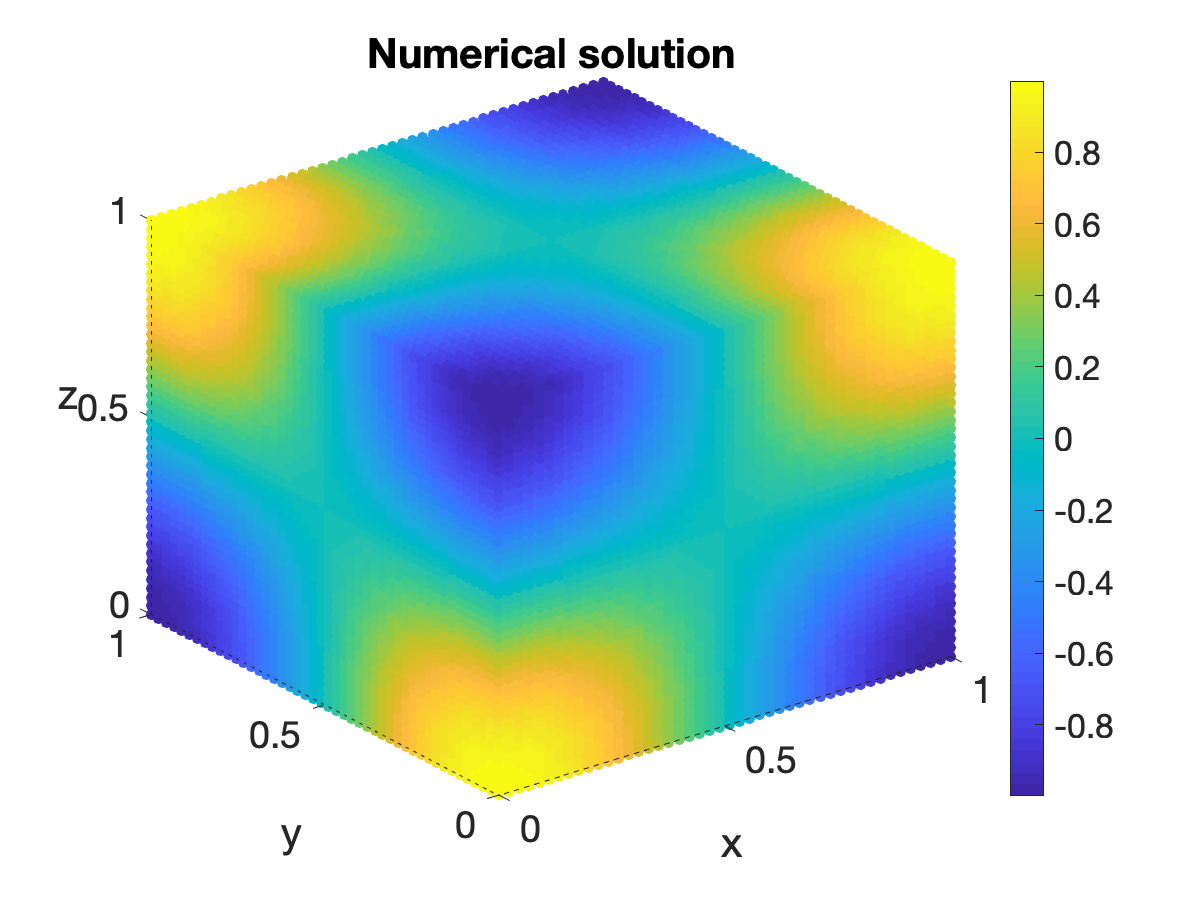
\includegraphics[scale=0.5]{laplace3dcube_numsol_Nx46.eps}
\end{center}
\caption{Poisson equation \eqref{experiment_laplace_equation_3d} on the unit cube $\Omega = [0,1]^3$: numerical solution obtained on the finest mesh for $i=9$ with $N= 97336$ nodes.}
\label{fig:laplace_3d_numsol}
\end{figure}

 
\subsubsection{Poisson equation on the sphere}
\label{sec:laplace_sphere}
We now consider another domain, the unit sphere $\Omega$ in 3D. The test problem, in spherical coordinates, is as follows
\begin{equation}
\label{experiment_laplace_equation_3d_sphere}
\begin{cases}
-&\Delta u + u = 4(3-5r^2) + (1-r^2)^2 \qquad \text{in}\ \Omega\\
&\nabla u \cdot \boldsymbol{n} = 0 \qquad \text{on}\ \partial \Omega
\end{cases}
\end{equation}
whose exact solution in spherical coordinates is given by
\begin{equation}
u(x,y,z) = (1-r^2)^2
\end{equation}
We consider a sequence of four cubic meshes $i=1,\dots,4$. The $i$-th mesh is obtained by subdividing each dimension into $5i$ intervals, thereby producing a cubic bounding mesh.  The cubic elements that are not fully contained in the sphere are then discarded. Finally, the outer faces of the resulting cubic mesh are extruded to fill the outer part of the sphere with irregular $8$-vertex polyhedra.  Such a mesh is shown in Fig.  \ref{fig:extruded_mesh_sphere}. On each mesh we solve the discrete problem,  we compute the error in $L^2(\Omega)$ norm and the respective convergence rate. As shown in Table \ref{tab:laplace_3d_convergence_sphere}, the convergence in $L^2(\Omega)$ norm is optimal, i.e. quadratic. The numerical solution obtained on the finest mesh is plotted in Fig.  \ref{fig:laplace_3d_numsol_sphere}.

\begin{figure}[H]
\begin{center}
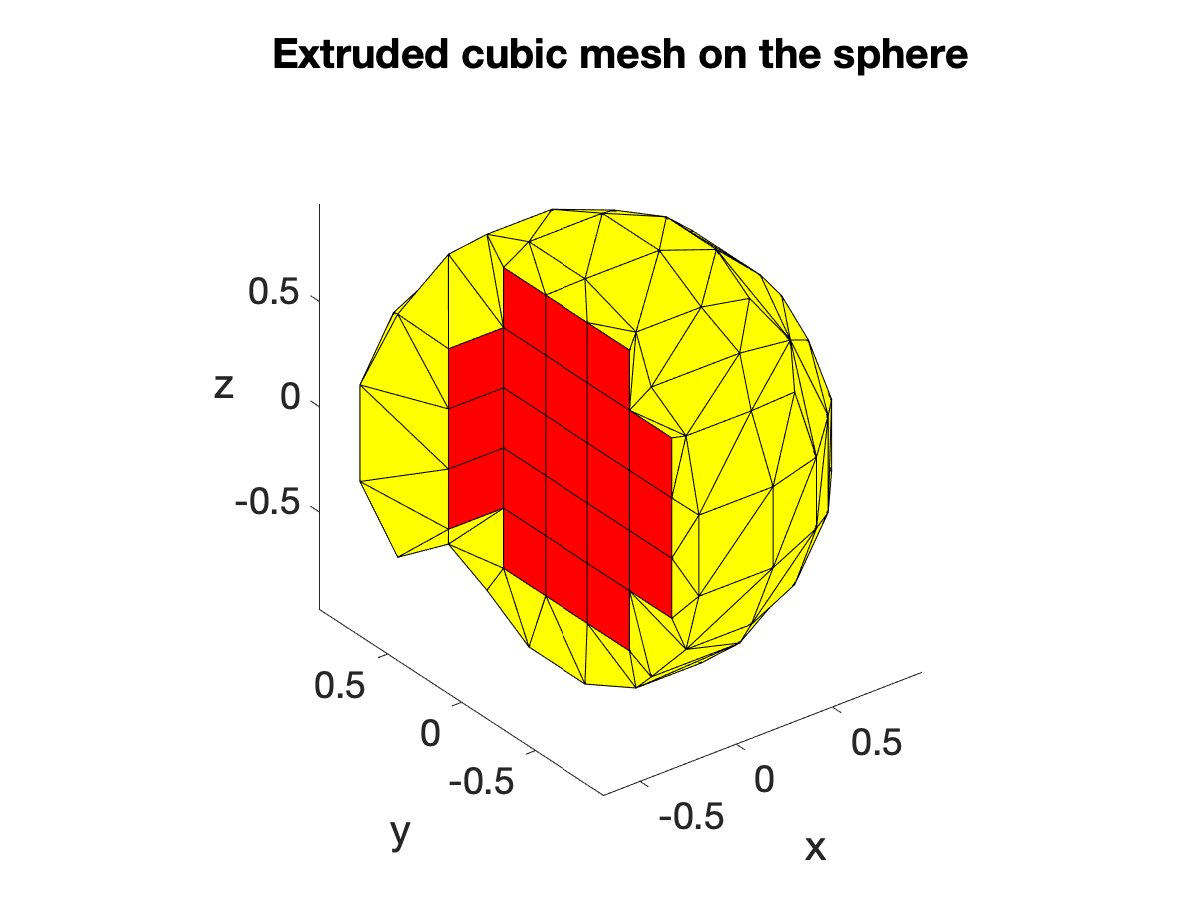
\includegraphics[scale=0.5]{extruded_mesh_sphere.eps}
\end{center}
\caption{Example of an extruded cubic mesh on the unit sphere.  The outermost elements, highlighted in yellow are irregular (but still star-shaped or even convex) $8$-vertex polyhedra.  The interior is filled with cubes (red).}
\label{fig:extruded_mesh_sphere}
\end{figure} 

\begin{table}[H]
\caption{Poisson equation \eqref{experiment_laplace_equation_3d_sphere} on the unit sphere $\Omega$ in 3D. The VEM implemented in VEMcomp shows optimal quadratic convergence in $L^2(\Omega)$ norm.}
\begin{center}
\begin{tabular}{c | c | c | c | c}
$i$ & $N$ & $h$ & $L^2(\Omega)$ error & $L^2(\Omega)$ rate\\
\hline
1 & 111 & 0.6928 &   1.3767 &  -   \\
2 & 799 & 0.3464 & 4.4137e-01 & 1.6412    \\
3 & 5749 & 0.1732 & 1.2532e-01 & 1.8164    \\
4 & 40381 & 0.0866 &  3.3139e-02 & 1.9190
\end{tabular}
\end{center}
\label{tab:laplace_3d_convergence_sphere}
\end{table}

\begin{figure}[H]
\begin{center}
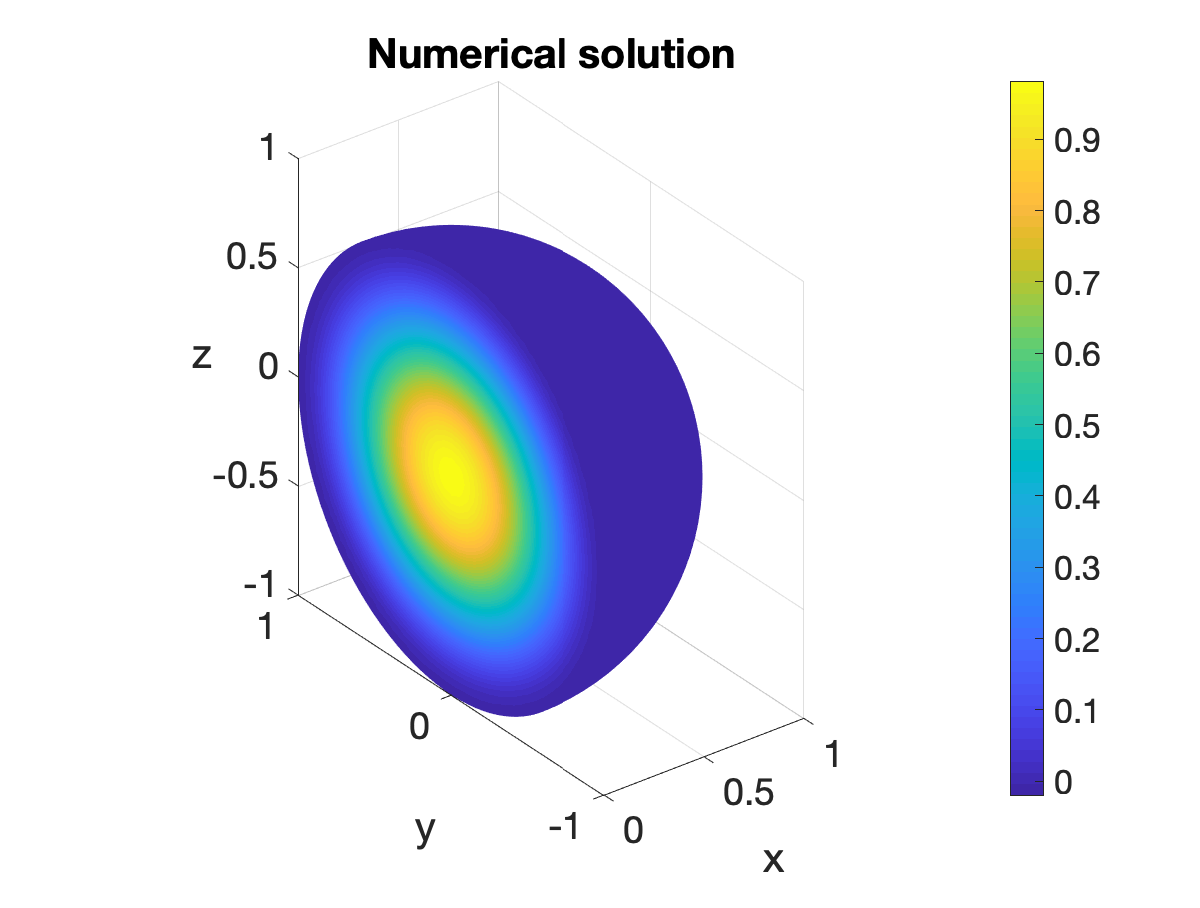
\includegraphics[scale=0.5]{laplace3dsphere_Nx41.eps}
\end{center}
\caption{Poisson equation \eqref{experiment_laplace_equation_3d_sphere} on the unit sphere $\Omega$ in 3D: numerical solution obtained on the finest mesh for $i=4$ with $N= 40381$ nodes.}
\label{fig:laplace_3d_numsol_sphere}
\end{figure} 

\subsection{Numerical examples for bulk-surface problems}
\red{We now apply VEMcomp to different types of BSPDEs.  In Example \ref{sec:example_elliptic_bs_sphere} we show a baseline problem given by a bulk-surface linear elliptic problem on the sphere. Example \ref{sec:example_parabolic_bs_sphere} introduces the time variable, by addressing the bulk-surface linear heat equation on the sphere.  In Example \ref{sec:example_bsrds_sphere}, we use VEMcomp to solve the top-end PDE problem considered in this work: a bulk-surface reaction-diffusion system (BSRDS) on the sphere.}

\subsubsection{Elliptic bulk-surface problem on the sphere}
\label{sec:example_elliptic_bs_sphere}
We numerically solve the following elliptic bulk-surface problem,  found in \cite{elliott2013finite}, on the unit sphere $\Omega$ in 3D:
\begin{equation}
\label{experiment_bs_3d_sphere}
\begin{cases}
-&\Delta u + u = xyz \qquad \text{in}\ \Omega\\
-&\Delta_\Gamma v + v +\nabla u\cdot\boldn = 29xyz \qquad \text{on}\ \partial \Omega\\
&\nabla u \cdot \boldn = -u + 2v   \qquad \text{on}\ \partial \Omega
\end{cases}
\end{equation}
whose exact solution is given by
\begin{align*}
&u(x,y,z) = xyz, \qquad (x,y,z) \in \Omega;\\
&v(x,y,z) = 2xyz, \qquad (x,y,z) \in \partial\Omega.
\end{align*}
We consider the same sequence of four meshes $\Omega_i$, $i=1,2,3,4$ of Experiment \ref{sec:laplace_sphere}.  The surface meshes are induced by the corresponding bulk mesh, i.e. $\Gamma_i = \partial \Omega_i$, $i=1,\dots,4$. On each mesh we solve the discrete problem,  we compute the error in $L^2(\Omega)\times L^2(\Gamma)$ norm and the respective convergence rate. As shown in Table \ref{tab:bs_3d_convergence_sphere}, the convergence in $L^2(\Omega)\times L^2(\Gamma)$ norm is optimal, i.e. quadratic. The numerical solution obtained on the finest mesh is plotted in Fig.  \ref{fig:bs_3d_numsol_sphere}.

\begin{table}[H]
\caption{Elliptic bulk-surface problem \eqref{experiment_bs_3d_sphere} on the unit sphere $\Omega$ in 3D. The VEM implemented in VEMcomp shows optimal quadratic convergence in $L^2(\Omega) \times L^2(\Gamma)$ norm. Times required for the solution of the linear system are shown.}
\begin{center}
\begin{tabular}{c | c | c | c | c | c}
$i$ & $N$ & $h$ & $L^2(\Omega)\times L^2(\Gamma)$ error & $L^2(\Omega)\times L^2(\Gamma)$ rate & Time (s)\\
\hline
1 & 111 & 0.6928 &   2.1985e-01 &  -   & 0.002159\\
2 & 799 & 0.3464 & 3.8387e-02 & 2.5178    & 0.015645\\
3 & 5749 & 0.1732 & 8.5674e-03 & 2.1637  & 0.197641  \\
4 & 40381 & 0.0866 &  1.9884e-03 & 2.1072 & 5.994934
\end{tabular}
\end{center}
\label{tab:bs_3d_convergence_sphere}
\end{table}

\begin{figure}[H]
\begin{center}
\hspace*{-10mm}
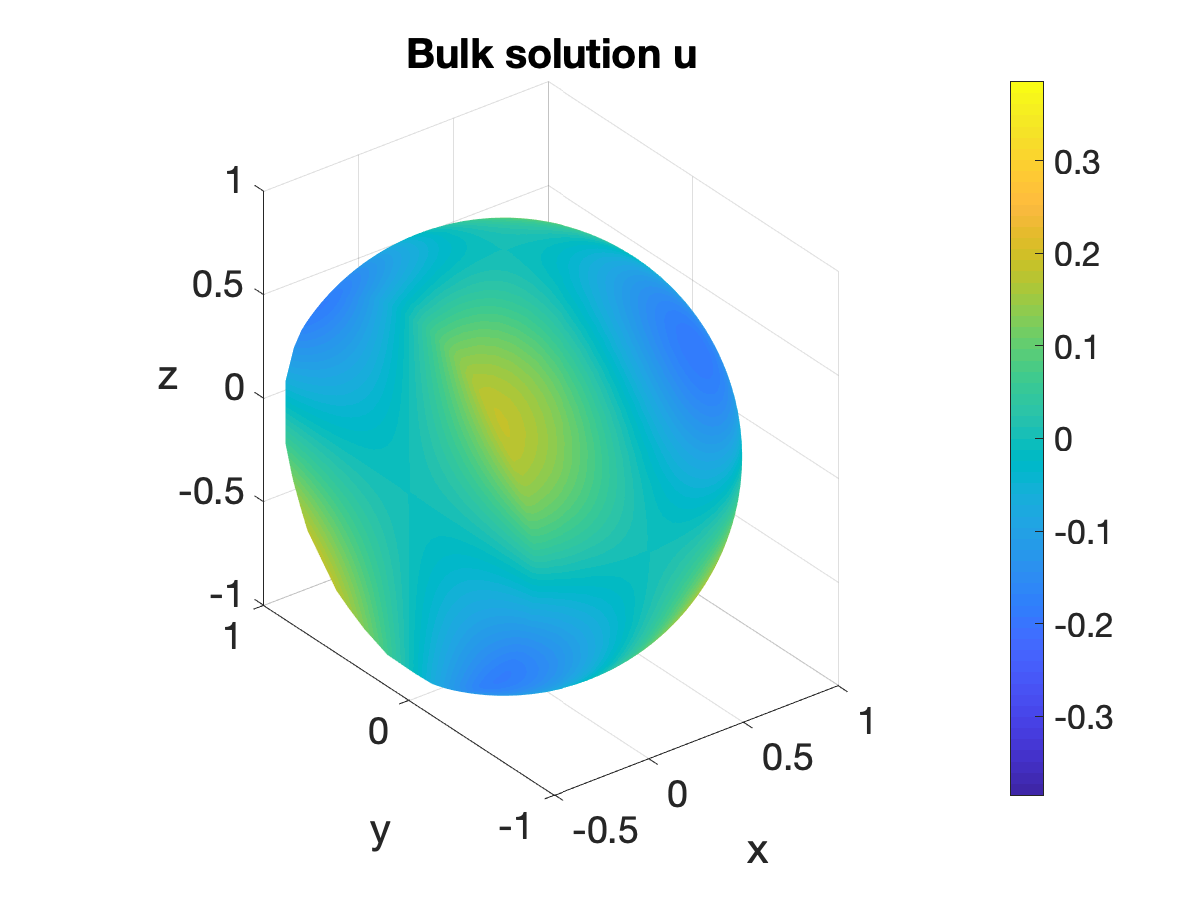
\includegraphics[scale=0.4]{bs_3d_sphere_nx41_u.eps}
\hspace*{-5mm}
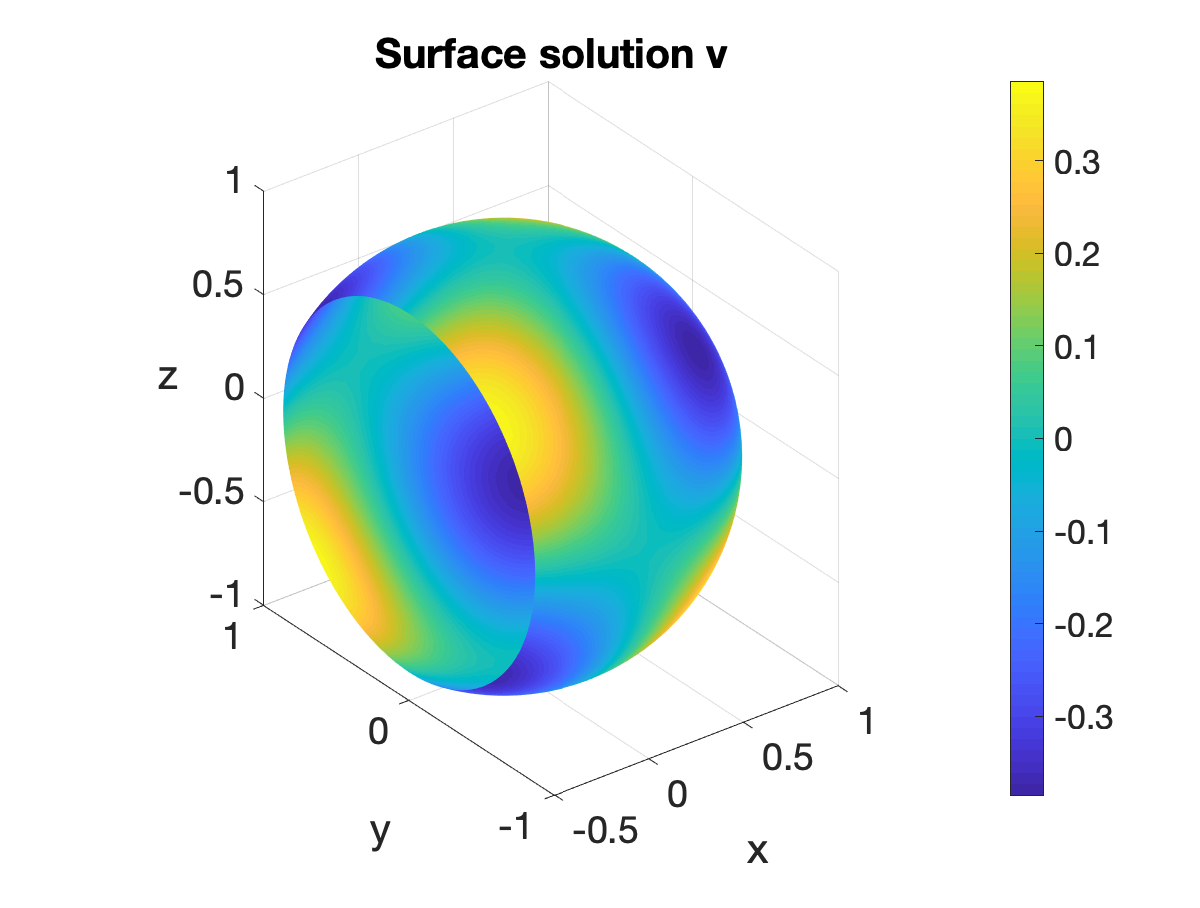
\includegraphics[scale=0.4]{bs_3d_sphere_nx41_v.eps}
\end{center}
\caption{Elliptic bulk-surface  problem \eqref{experiment_bs_3d_sphere} on the unit sphere $\Omega$ in 3D: numerical solution obtained on the finest mesh for $i=4$ with $N= 40381$ nodes. Left: bulk component $u$. Right: surface component $v$.}
\label{fig:bs_3d_numsol_sphere}
\end{figure} 

\subsubsection{Parabolic bulk-surface problem on the sphere}
\label{sec:example_parabolic_bs_sphere}
We numerically solve the following parabolic bulk-surface problem,  found in \cite{frittelli2021bulk}, on the unit sphere $\Omega$ in 3D:
\begin{equation}
\label{experiment_bs_3d_sphere_parabolic}
\begin{cases}
&\dot{u} -\Delta u  = xyze^t \qquad  \text{in}\ \Omega \times [0,T];\\
&\dot{v} -\Delta_\Gamma v +\nabla u\cdot\boldn = 16xyze^t \qquad \text{on}\ \partial \Omega \times [0,T];\\
&\nabla u \cdot \boldn = 3xyze^t  \qquad \text{on}\ \partial \Omega \times [0,T],
\end{cases}
\end{equation}
for final time $T=1$, whose exact solution is given by
\begin{align*}
&u(x,y,z,t) = xyze^t, \qquad (x,y,z,t) \in \Omega \times [0,T];\\
&v(x,y,z,t) = 2xyze^t, \qquad (x,y,z,t) \in \partial\Omega \times [0,T].
\end{align*}
We consider the same sequence of four meshes $\Omega_i$, $i=1,2,3,4$ of Experiment \ref{sec:example_elliptic_bs_sphere}.  Correspondingly, we choose timesteps $\tau_i = 2^{1-i}$,  $i=1,2,3,4$. On each mesh we solve the discrete problem,  we compute the error in $L^2(\Omega)\times L^2(\Gamma)$ norm at the final time $T=1$ and the respective convergence rate. As shown in Table \ref{tab:bs_3d_convergence_sphere_parabolic}, the convergence in $L^2(\Omega)\times L^2(\Gamma)$ norm is optimal, i.e. quadratic in space and linear in time. The numerical solution at the final time obtained on the finest mesh is plotted in Fig.  \ref{fig:bs_3d_numsol_sphere_parabolic}.

\begin{table}[H]
\caption{Parabolic bulk-surface problem \eqref{experiment_bs_3d_sphere_parabolic} on the unit sphere $\Omega$ in 3D. The VEM implemented in VEMcomp shows optimal quadratic convergence in $L^2(\Omega) \times L^2(\Gamma)$ norm. Times required for the time integration are shown.}
\begin{center}
\begin{tabular}{c | c | c | c | c | c | c}
$i$ & $N$ & $h$ & $\tau$ & $L^2(\Omega)\times L^2(\Gamma)$ error & $L^2(\Omega)\times L^2(\Gamma)$ rate & Time (s)\\
\hline
1 & 111 & 0.6928 &   1 & 1.2074 &  -   & 0.002417\\
2 & 799 & 0.3464 & 2.5e-1 & 4.3481e-01 & 1.4734    & 0.038881\\
3 & 5749 & 0.1732 & 6.25e-2 & 1.2110e-01 & 1.8442  & 2.134601  \\
4 & 40381 & 0.0866 &  1.5625e-2 & 3.0881e-02 & 1.9714 & 287.345570
\end{tabular}
\end{center}
\label{tab:bs_3d_convergence_sphere_parabolic}
\end{table}

\begin{figure}[H]
\begin{center}
\hspace*{-10mm}
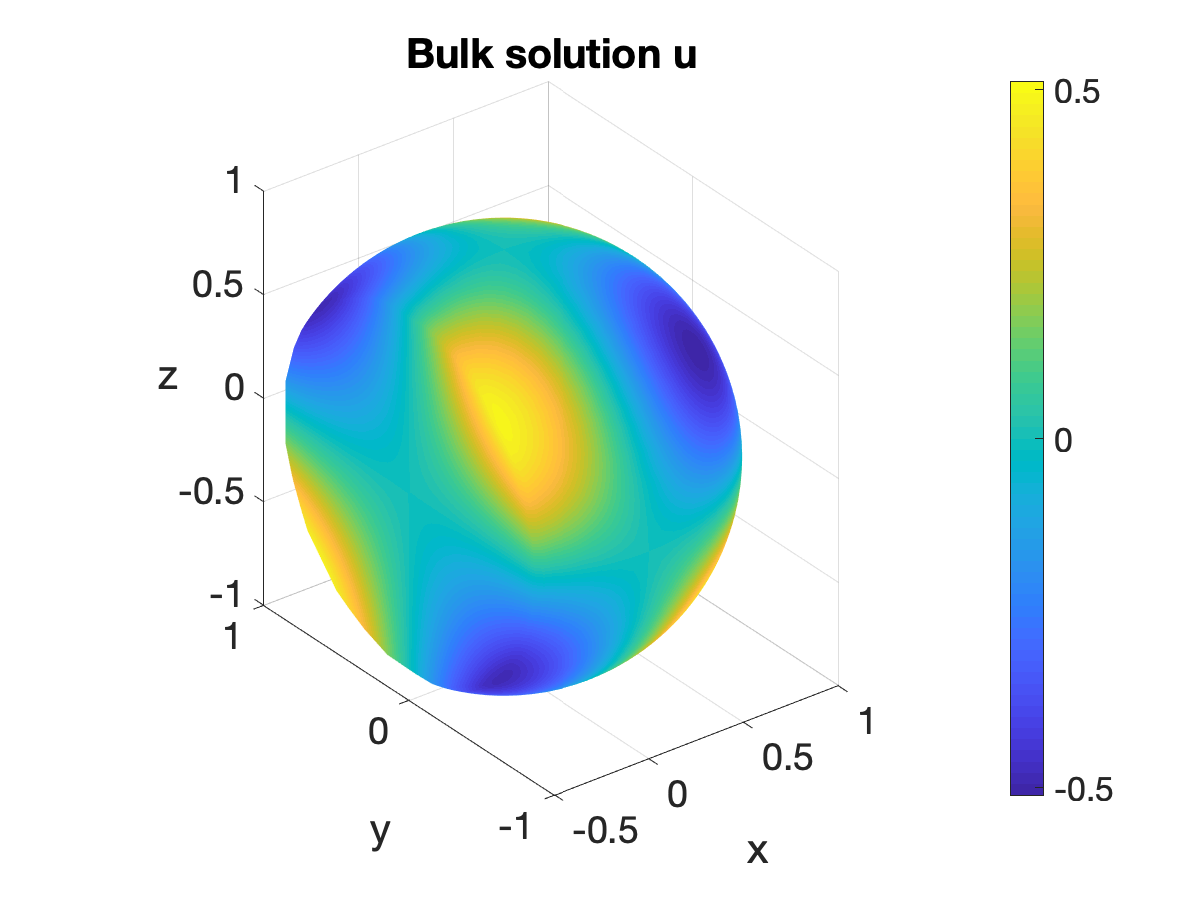
\includegraphics[scale=0.4]{bs_3d_sphere_nx41_parabolic_u.eps}
\hspace*{-5mm}
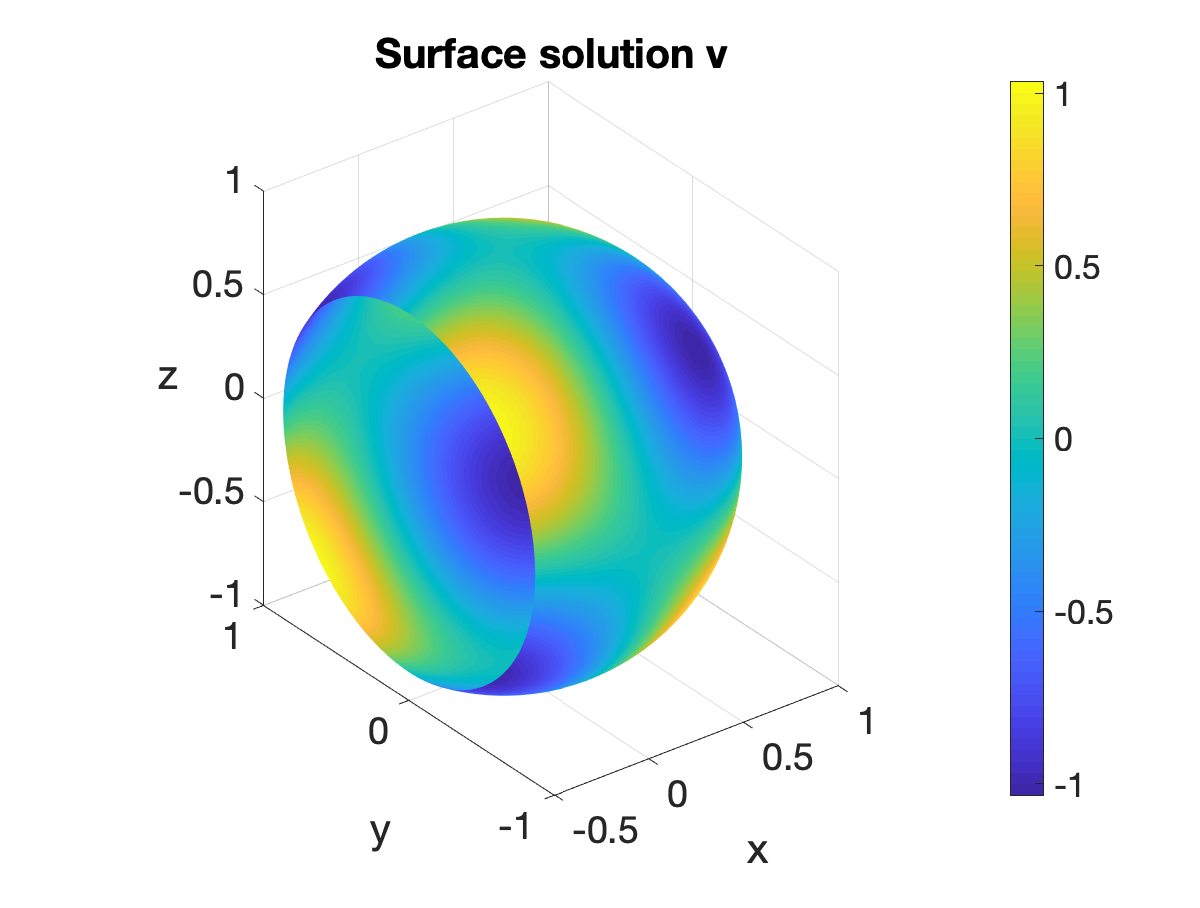
\includegraphics[scale=0.4]{bs_3d_sphere_nx41_parabolic_v.eps}
\end{center}
\caption{Parabolic bulk-surface  problem \eqref{experiment_bs_3d_sphere_parabolic} on the unit sphere $\Omega$ in 3D: numerical solution obtained on the finest mesh for $i=4$ with $N= 40381$ nodes and timestep $\tau = 1.5625e-2$. Left: bulk component $u$. Right: surface component $v$.}
\label{fig:bs_3d_numsol_sphere_parabolic}
\end{figure} 

\subsubsection{\red{Bulk-surface reaction-diffusion system on the sphere}}
\label{sec:example_bsrds_sphere}
\red{In this final example we solve the following BSRDS considered in \cite{frittelli2023bsrds}.}
 
\bibliographystyle{plainurl}
\bibliography{bibliography}
 

\end{document}